\documentclass[a4paper,11pt]{article}
\usepackage{jcappub}
\usepackage{bm}
\usepackage{booktabs}
\usepackage{array}
\usepackage{orcidlink}
\hypersetup{pdftitle={Peaks or thresholds? Non-Gaussian primordial black hole abundances for broad
spectra and the pulsar-timing-array tension},pdfauthor={Duong Ngoc Khoa}}
\graphicspath{{figures/}}
\setlength{\emergencystretch}{1.5em}

\newcommand{\Cg}{C_{\rm g}}
\newcommand{\Cl}{C_{\ell}}
\newcommand{\zr}{\zeta_r}
\newcommand{\zg}{\zeta_{\rm g}}
\newcommand{\dd}{\mathrm{d}}
\newcommand{\E}{\mathbb{E}}
\newcommand{\fnl}{f_{\rm NL}}
\newcommand{\fpbh}{f_{\rm PBH}}
\newcommand{\Mo}{M_\odot}
\newcommand{\Pz}{\mathcal{P}_\zeta}

\title{Peaks or thresholds? Non-Gaussian primordial black hole abundances for broad spectra and
the pulsar-timing-array tension}

\author{Duong Ngoc Khoa\,\orcidlink{0009-0009-9409-3298}}
\affiliation{Phenikaa Institute for Advanced Study, Phenikaa University, Hanoi, Vietnam}
\emailAdd{yuutoduong@gmail.com}

\abstract{Primordial black holes (PBHs) from a peak in the curvature spectrum are counted either
with threshold statistics or with peaks theory. With local non-Gaussianity (NG), peaks theory had
been applied only to monochromatic spectra or with the peak condition imposed on a Gaussian field.
We construct it on the compaction function for broad spectra, as the exact counterpart of
threshold statistics. Maxima of the non-Gaussian compaction $\Cl=F'(\zr)\Cg$ are maxima of the
Gaussian field $\Cg+\lambda\zr$, times a rank-one Hessian factor that we compute to first order; a
Monte Carlo and counts on $256^3$ lattices confirm it, and show that the Gaussian-peak approximation
miscounts peaks by up to 18\%. The amplitude ratio
$R=A_*^{\rm peaks}/A_*^{\rm threshold}$ is 0.74--0.82 for $|\fnl|\le2$ and lognormal widths
0.1--2, and NG cancels in $R/R_{\rm Gauss}$ to about 4\% (16\% for a strong ultra-slow-roll tail),
so one function of the width converts threshold-statistics results to peaks theory. For the NANOGrav 15-year data, peaks theory
strengthens the exclusion of a scalar-induced gravitational-wave explanation by 0.2--0.8$\sigma$
for every NG template, or by 0.04--0.39$\sigma$ with a background from supermassive black hole
binaries, which caps the exclusion at $2.8\sigma$. Primordial NG in the induced gravitational
waves, with all seven terms, lowers the significance by up to $0.26\sigma$ and leaves this shift
unchanged. Three rarely stated analysis choices matter as much as the statistics: the frequency
range, when the transfer function acts in the collapse threshold, and the normalisation of
$\fpbh$, which the expression in common use overestimates by a factor of 3--13.}

\keywords{primordial black holes, non-gaussianity, gravitational waves / theory, physics of the
early universe}

\begin{document}
\maketitle
\flushbottom

\section{Introduction}\label{sec:intro}

Pulsar timing arrays (PTAs) have found evidence for a nanohertz gravitational-wave (GW)
background \cite{NG15gwb,EPTA23,PPTA23,CPTA23}. One cosmological interpretation is the GWs
induced at second order by a peak in the primordial curvature spectrum
\cite{Ananda,Baumann,Kohri,Domenech,NG15np,FPRS23,Ellis23}. A peak large enough to produce the
signal also forms primordial black holes (PBHs) when the perturbations re-enter the horizon, and
requiring that PBHs are not overproduced disfavours the scenario at the 2--3$\sigma$ level
\cite{FIVT23,NG15np,Iovino24}. How strongly depends on the non-Gaussianity (NG) of the curvature
perturbation \cite{FIVT23,LCH23,WZLZ23} and on how the PBH abundance is computed \cite{Iovino24}.

Two prescriptions are in use for the abundance (see ref.~\cite{CIPVV26} for a review). Threshold
statistics counts the volume fraction in which the compaction function \cite{SS99,Harada15}
exceeds a threshold; it includes the non-linear relation between curvature and density
\cite{Young19,DeLuca19} and any local NG non-perturbatively \cite{Ferrante,Ianniccari}. Peaks
theory counts maxima instead \cite{BBKS,Yoo18}. It has been developed for Gaussian curvature
perturbations with spectra of finite width \cite{Yoo20,GS20,Pi25,Kushwaha,ColeFumagalli} and, with
local NG, either for monochromatic spectra \cite{Young22,Kitajima,Inui} or with the peak condition
imposed on the Gaussian component \cite{AGM19,YGY19,Riccardi}. For Gaussian curvature
perturbations the two prescriptions have been compared in refs.~\cite{Gow21,Ianniccari,Kushwaha,Iovino24}.
Several recent papers state that peaks theory with local NG for broad spectra is an open problem
\cite{Ianniccari,Iovino24,IPV25,Pi25,ColeFumagalli,GTV25}, and Franciolini et al.~\cite{FIVT23}
note that peaks theory ``provides slightly smaller amplitudes'', so that their threshold-statistics
bounds are conservative.

This paper fills that gap and quantifies their remark. In section~\ref{sec:stats} we build peaks
theory on the compaction function for broad spectra with local NG (quadratic, logarithmic or
ultra-slow-roll, and curvaton templates), as the exact counterpart of threshold statistics, so
that the two differ only by the peak condition. The main technical step is to count maxima of the
non-Gaussian compaction itself, a local function of two correlated Gaussian fields, rather than
of its Gaussian component. Section~\ref{sec:abund} sets out the conventions for the abundance.
Section~\ref{sec:R} gives the amplitude ratio $R(\Delta,{\rm NG})$ between the statistics, and
section~\ref{sec:pta} propagates it to the significance of the PBH-overproduction tension for
NANOGrav 15, with every analysis choice stated and varied. There we also add the primordial-NG
corrections to the GW spectrum \cite{CPS19,Unal19,ALW21}, which ref.~\cite{FIVT23} neglects, and an
astrophysical background. Section~\ref{sec:disc} discusses the results and their limitations,
and section~\ref{sec:concl} concludes.

Two conventions turn out to matter, and the second is widespread in the literature. The collapse
threshold of ref.~\cite{FIVT23} follows the superhorizon smoothing of Musco et al., in effect
without a transfer function, although their formula is written with the horizon-crossing transfer
function; read that way, it changes the amplitude by 18--62\% (section~\ref{sec:abund} and
appendix~\ref{app:th}). The normalisation of $\fpbh$ in common use is too large by a factor of
3--13 (appendix~\ref{app:fpbh}).

Our construction differs from the closest existing work as follows. Yoo, Gong and Yokoyama
\cite{YGY19} count peaks of $\zg$ with typical profiles and quadratic NG, assuming that every peak
of $\zg$ is a peak of $\zeta$, which holds for $\frac35\fnl\gtrsim-\frac14$. Riccardi et
al.~\cite{Riccardi} treat quadratic NG for finite-width spectra with peaks of the curvature
perturbation and the linear relation between density and curvature, not the compaction function.
Escriv\`a \cite{Escriva26} counts peaks of $\zg$ for the logarithmic template and adds a
dispersion of the profile shape, which for negative NG and broad spectra raises the abundance by
orders of magnitude. Germani et al.~\cite{Germani25} give the statistics of peaks of general
local-NG fields and apply it to their sphericity. None of these compares with threshold statistics
in the same conventions. We count maxima of the non-Gaussian compaction itself, with the
threshold, window, transfer function and cut of threshold statistics, so that $R$ isolates the
peak condition.

\section{Two statistics for the non-Gaussian compaction}\label{sec:stats}

\subsection{Local NG and the compaction function}

The curvature perturbation is $\zeta=F(\zg)$ with $\zg$ Gaussian and power spectrum $\Pz$. We use
three templates: the quadratic $F=\zg+\frac35\fnl\zg^2$; the ultra-slow-roll (USR) logarithm
$F=-\mu_*\ln(1-\zg/\mu_*)$ \cite{AGM19}, which is the $F=-\frac2\beta\ln(1-\frac\beta2\zg)$ of
ref.~\cite{FIVT23} with $\mu_*=2/\beta$ and has $\fnl=5/(6\mu_*)$ at second order; and the
sudden-decay curvaton, $\zeta=\ln X(r_{\rm dec},\zg)$ \cite{SVW06,Ferrante}. For the curvaton, $X$
depends on $\zg$ only through $(1+3\zg/2r_{\rm dec})^2=(\sigma/\bar\sigma)^2$, with $\sigma$ the
curvaton field, so troughs of $\zg$ below $-2r_{\rm dec}/3$, where $\sigma$ changes sign, are also
peaks of $\zeta$. For $r_{\rm dec}<1$ we integrate both branches.

We use two spectral shapes, a lognormal of width $\Delta$ and the broken power law
BPL($\alpha,\beta,\gamma$) of ref.~\cite{FIVT23}:
\begin{equation}
\Pz=\frac{A}{\sqrt{2\pi}\,\Delta}\exp\Big[-\frac{\ln^2(k/k_*)}{2\Delta^2}\Big],\qquad
\Pz=A\,\frac{(\alpha+\beta)^\gamma}{\big[\beta(k/k_*)^{-\alpha/\gamma}+\alpha(k/k_*)^{\beta/\gamma}\big]^\gamma}.
\label{eq:spectra}
\end{equation}
$A$ is the integrated power of the lognormal and the peak value of the BPL. The slopes
$\alpha,\beta$ and the width $\gamma$ of the BPL are not to be confused with the mass fraction and
the critical exponent used below. At smoothing scale $r$, the scale that re-enters the horizon at
formation ($k=1/r$), we define the Gaussian fields
\begin{align}
\Cg(\bm x;r)&=\int\!\frac{\dd^3k}{(2\pi)^3}e^{i\bm k\cdot\bm x}\,\tfrac{2\Phi}{3}(kr)^2W(kr)T(kr)\,\zg(\bm k),\\
\zr(\bm x;r)&=\int\!\frac{\dd^3k}{(2\pi)^3}e^{i\bm k\cdot\bm x}\,W_s(kr)T(kr)\,\zg(\bm k),
\end{align}
with the top-hat window $W(y)=3(\sin y-y\cos y)/y^3$, the shell window $W_s(y)=\sin y/y$, the
radiation transfer function $T(y)=W(y/\sqrt3)$ and $\Phi=2/3$. All moments use a hard cut
$kr<4.49$, the first zero of $W$, as in \texttt{pbhstat} \cite{ColeFumagalli}. With the transfer
function the moments of the spectra used here also converge without the cut, which changes
threshold-statistics amplitudes by $\le2.3\%$ and hardly affects the ratio between the statistics
(section~\ref{sec:R}). For a spherical configuration $\Cg=-2\Phi r\zg'$ and $\zr=\zg(r)$, and the
linear and full compaction of $\zeta=F(\zg)$ are \cite{Young19,DeLuca19,Ferrante,Young22}
\begin{equation}
\Cl=F'(\zr)\,\Cg,\qquad C=\Cl-\frac{\Cl^2}{4\Phi}.
\label{eq:Cl}
\end{equation}
A PBH of mass $M=\mathcal K(C-C_{\rm th})^\gamma M_H$ \cite{EC94,NJ98,MM13} forms where
$C>C_{\rm th}$ and $\Cl<2\Phi$ (type I). We use $\mathcal K=3.3$ and $\gamma=0.36$, as in
refs.~\cite{Ferrante,Ianniccari}. The threshold $C_{\rm th}=\delta_c(q)$ follows the
shape-dependent prescription of Musco et al.~\cite{Musco19,EGS20,Musco21}, with the transfer
function in the moments.

\subsection{Threshold statistics}

With $P_{\rm G}(c,z)$ the bivariate Gaussian of $(\Cg,\zr)$, the mass fraction at one scale is
\cite{Ferrante}
\begin{equation}
\beta_{\rm th}=\int\dd z\int_{C_{\ell,\rm th}}^{2\Phi}\dd\Cl\;\frac{P_{\rm G}(\Cl/F'(z),z)}{|F'(z)|}\;
\mathcal K(C-C_{\rm th})^\gamma ,
\label{eq:betath}
\end{equation}
where $C_{\ell,\rm th}=2\Phi[1-(1-C_{\rm th}/\Phi)^{1/2}]$. Equation~\eqref{eq:betath} includes the
non-linear relation $C(\Cl)$ and the full $F$.

\subsection{Peaks of the Gaussian component (Gaussian-peak approximation)}

The natural generalisation of earlier work is to count BBKS maxima of the Gaussian field $\Cg$,
with $\zr$ as a correlated scalar, and to map them through $F'$; where $F'<0$, maxima of $\Cl$ are
minima of $\Cg$. This replaces the volume weight in eq.~\eqref{eq:betath} by
\begin{equation}
w=\frac{V\,G(m,s)}{(2\pi)^{3/2}R_*^3},\qquad G(m,s)=\int_0^\infty\dd x\,f(x)\,\mathcal N(x;m,s^2),
\qquad V=\tfrac43\pi r^3,
\label{eq:3a}
\end{equation}
where $f$ is the BBKS function \cite{BBKS}, $m$ and $s^2$ are the conditional mean and variance
of $x=-\nabla^2\Cg/\sigma_{2}$ given $(\Cg,\zr)$, and $R_*=\sqrt3\sigma_1/\sigma_2$. This is exact
for constant $F'$, but not in general: $\nabla\Cl=F'\nabla\Cg+F''\Cg\nabla\zr$, so the maxima of
$\Cl$ are displaced from those of $\Cg$.

\subsection{Peaks of the non-Gaussian compaction}

The Kac--Rice density of maxima of $\Cl$ at $(\Cg,\zr)=(c,z)$ follows in three steps. First, the
gradient factorises,
\begin{equation}
\nabla\Cl=F'(z)\,\nabla Y_\lambda,\qquad Y_\lambda\equiv\Cg+\lambda\zr,\qquad \lambda=\frac{cF''(z)}{F'(z)},
\end{equation}
with $\lambda$ frozen at the point, so that $Y_\lambda$ is a Gaussian field. Second, at a
stationary point the Hessian is $\nabla\nabla\Cl=F'[\nabla\nabla Y_\lambda+\kappa\nabla\zr\nabla\zr^T]$,
with $\kappa=-cF'(1/F')''$; the rank-one term vanishes identically for the USR template, for which
$1/F'$ is linear. Third, conditional on $\nabla Y_\lambda=0$, the gradient $\nabla\zr$ is Gaussian
with variance $v=(\sigma^2_{1,cc}\sigma^2_{1,rr}-\sigma^4_{1,cr})/(3\sigma^2_{1,\lambda})$, where
$\sigma^2_{n,AB}=\int\dd\ln k\,k^{2n}K_AK_B\Pz$ and
$\sigma^2_{n,\lambda}=\sigma^2_{n,cc}+2\lambda\sigma^2_{n,cr}+\lambda^2\sigma^2_{n,rr}$. The matrix
determinant lemma then gives the peak density exactly to first order in
$\tau=s\kappa v/\sigma_{2,\lambda}$ (appendix~\ref{app:3b}):
\begin{equation}
\boxed{\;n(c,z)=P_{\rm G}(c,z)\,\frac{G(s\,m_\lambda,s_\lambda)}{(2\pi)^{3/2}R_{*,\lambda}^3}\,
\big[1-\tau R_2(s\,m_\lambda,s_\lambda)\big],\qquad R_{*,\lambda}=\frac{\sqrt3\,\sigma_{1,\lambda}}{\sigma_{2,\lambda}},\;}
\label{eq:3b}
\end{equation}
with $s={\rm sign}\,F'$, $m_\lambda$ and $s_\lambda$ the conditional moments of
$-\nabla^2Y_\lambda/\sigma_{2,\lambda}$, and $R_2=27\int f_2\mathcal N/\int f\mathcal N\to9/m$. The
peak mass fraction is eq.~\eqref{eq:betath} with the integrand multiplied by $Vn/P_{\rm G}$.
Equation~\eqref{eq:3b} reduces to eq.~\eqref{eq:3a} for $\lambda=0$ (Gaussian $\zeta$ or $F''=0$)
and for a monochromatic spectrum, where $Y_\lambda\propto\zr$, and it stays finite as $F'\to0$.
The rank-one factor is formally one power of the r.m.s.\ amplitude smaller, but
$\kappa=-2\lambda^2/c$ for the quadratic template, and it changes the local density by up to 36\%
at nodes with $\fnl=-2$, $\Delta=1$.

We checked eq.~\eqref{eq:3b} in two independent ways. A Monte Carlo of the 20 Gaussian variables
with the exact Hessian reproduces it to $3\times10^{-4}$ at 15 of 16 test nodes, and to 0.85\% at
the most extreme one. We also counted local maxima of $\Cl$ on $256^3$ Gaussian random fields
(lognormal $\Delta=1$, 24 realisations), with predictions from the lattices' own mode sums
(figure~\ref{fig:lattice}). Equation~\eqref{eq:3b} follows the counts to about 1\% beyond the grid
trend seen in the Gaussian case, while the Gaussian-peak approximation~\eqref{eq:3a} is off by up
to 18\% for $\fnl=-2$.

\begin{figure}[t]
\centering
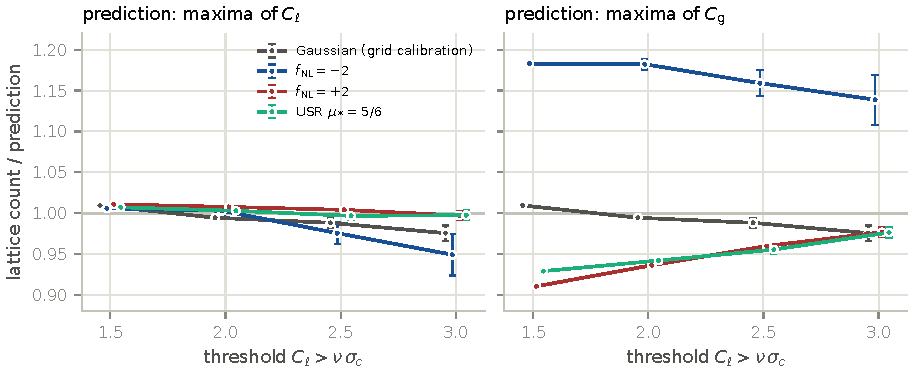
\includegraphics[width=\textwidth]{fig_phase3b_lattice}
\caption{Test of the peak density on lattices. Maxima of the non-Gaussian compaction
$\Cl=F'(\zr)\Cg$ above the threshold $\nu\sigma_c$, counted on 24 Gaussian random fields of
$256^3$ points (lognormal spectrum, $\Delta=1$, smoothing scale $r=8$ cells, $\sigma_c=0.15$,
$k<4.49/r$), divided by the prediction of eq.~\eqref{eq:3b} (left) and of the Gaussian-peak
approximation~\eqref{eq:3a} (right), for quadratic NG with $\fnl=\pm2$ and the USR template with
$\mu_*=5/6$. Both predictions use the lattices' own mode sums. Gray: Gaussian $\zeta$, whose
departure from 1 calibrates the grid.}
\label{fig:lattice}
\end{figure}

\section{Abundance and its conventions}\label{sec:abund}

The abundance integrates the mass fraction over the horizon mass $M_H$ at which $k=1/r$
re-enters,
\begin{equation}
\fpbh=\int\dd\ln M_H\;w(M_H)\,\beta(M_H),
\label{eq:fpbh}
\end{equation}
and three normalisations of the weight $w$ are in use (appendix~\ref{app:fpbh}):
\begin{equation}
w=\frac{1}{\Omega_{\rm DM}}\Big(\frac{M_{\rm eq}}{M_H}\Big)^{1/2}
\quad\text{or}\quad
w=\frac{1}{\Omega_{\rm DM}}\Big(\frac{M_H}{\Mo}\Big)^{-1/2}\Big(\frac{g_*}{106.75}\Big)^{3/4}
\Big(\frac{g_{*s}}{106.75}\Big)^{-1}\frac{1}{c_w}.
\label{eq:w}
\end{equation}
The first is the $M_{\rm eq}$ form of refs.~\cite{Ferrante,ColeFumagalli}. The second is eq.~(14)
of ref.~\cite{FIVT23} for $c_w=7.9\times10^{-10}$, and the first-principles result from entropy
conservation for $c_w=1.0\times10^{-8}$. The first two overestimate $\fpbh$ by factors of 3--5
and 12.7, respectively. Since $\beta$ depends exponentially on $1/A$, this lowers the amplitude
for $\fpbh=1$ by only $\ln(\text{factor})/|\ln\beta|\simeq8\%$ and 12\%. These factors cancel in
$R$ but not in the PTA tension.

The threshold prescription is a second, larger choice. The shape parameter $q$ of Musco et
al.~\cite{Musco21} is computed from the spectrum smoothed with the transfer function $T(k,\eta)$,
and it matters when $T$ acts. Musco et al.\ apply it on superhorizon scales, $\hat r_m\simeq10\,r_H$,
where $T\simeq1$ except for modes with $k\hat r_m\gtrsim20$; for every spectrum used here this
agrees with no transfer function to $\le0.0005$ in $\delta_c$. Applied at horizon crossing, as in
the variances, it smooths much more: for a lognormal of width $\Delta=1$ it gives $\delta_c=0.537$
instead of $0.458$, and for the broken power law of ref.~\cite{FIVT23} ($\alpha,\beta,\gamma=4,3,1$)
it gives $0.570$ instead of $0.544$. Ref.~\cite{FIVT23} writes the horizon-crossing $T(k,r_m)$ in
its eqs.~(S4)--(S5), but its figure~S3 follows the superhorizon prescription over its whole range
(appendix~\ref{app:th}). The two readings move $A_*$ by 18\% (BPL) and 62\% (lognormal, $\Delta=1$)
for every statistic, because the linear threshold $C_{\ell,\rm th}$ grows faster than $C_{\rm th}$.
They hardly affect the ratio between the statistics: $R$ changes by $\le0.5\%$ for quadratic NG
and by $\le6\%$ for the curvaton and strong USR tails. Sections~\ref{sec:stats}--\ref{sec:R} use
the horizon-crossing threshold, and section~\ref{sec:pta} uses both. Table~\ref{tab:conv} collects
the conventions of the two analyses.

\begin{table}[t]
\centering\small
\begin{tabular}{@{}>{\raggedright\arraybackslash}p{3.2cm}>{\raggedright\arraybackslash}p{5.4cm}>{\raggedright\arraybackslash}p{6.0cm}@{}}
\toprule
 & ratio $R$ (sections~\ref{sec:stats}--\ref{sec:R}) & PTA tension (section~\ref{sec:pta})\\
\midrule
windows & top-hat $W$ for $\Cg$, shell $W_s$ for $\zr$ & same\\
transfer function in the moments & $T(kr)$, radiation & same\\
UV cut of the moments & $kr<4.49$ & same\\
collapse & $\mathcal K=3.3$, $\gamma=0.36$, type I & same\\
threshold $C_{\rm th}$ & Musco et al., $T$ at horizon crossing & Musco et al.\ without $T$, as in
ref.~\cite{FIVT23}; with $T$ as a variant\\
peaks & maxima of $\Cl$, BBKS, $V=\frac43\pi r^3$ & same\\
$\fpbh$ normalisation & $M_{\rm eq}$ form, eq.~\eqref{eq:w} & eq.~(14) of ref.~\cite{FIVT23}; entropy
conservation as a variant\\
target abundance & $\fpbh=1$ & $\fpbh=1$; $10^{-3}$ as a variant\\
spectra & lognormal, $\Delta=0.1$--2, $k_*=10^7\,{\rm Mpc}^{-1}$; BPL($4,\beta,1$), $\beta=2$--4 &
BPL(4,3,1); lognormal, $\Delta=0.5$, 1, 2\\
GW spectrum & --- & Gaussian $\zeta$; NG terms in section~\ref{sec:ngsigw}\\
PTA data & --- & NANOGrav 15, lowest 14 bins, KDEs blurred by 0.05 dex\\
priors & --- & uniform in $\log_{10}k_*\in[5,10]$ and $\log_{10}A\in[-3,0]$\\
astrophysical background & --- & none; SMBHBs in section~\ref{sec:smbhb}\\
\bottomrule
\end{tabular}
\caption{Conventions of the two analyses. The threshold, window, transfer function, cut,
$\mathcal K$, $\gamma$ and $\fpbh$ normalisation are always the same for threshold statistics and
peaks theory, so that the comparison between them is like-for-like.}
\label{tab:conv}
\end{table}

Our implementation, \texttt{ngpbh}, reproduces the public code \texttt{pbhstat}
\cite{ColeFumagalli} in its conventions to 0.017\% in $A_*$ for $\Delta=0.1$--2, for both
statistics. It also reproduces the broad-spectrum benchmark of Ferrante et al.\ (amplitude
$9.09\times10^{-3}$ against $9.2\times10^{-3}$) and their curvaton amplitudes to 1\%
\cite{Ferrante}. The integration uses Gauss--Legendre nodes in $\Cl$ that absorb the
$(C-C_{\rm th})^\gamma$ cusp and an adaptive window in $\zr$, all in $\log\beta$, and it is stable
to $10^{-5}$ when every grid is doubled.

\section{The gap between the statistics, with NG}\label{sec:R}

Table~\ref{tab:R} and figure~\ref{fig:R} give $R=A_*^{\rm peaks}/A_*^{\rm threshold}$ for
$\fpbh=1$, with the same threshold, window, transfer function, cut, $\mathcal K$ and $\gamma$ for
both statistics. For Gaussian $\zeta$, $R=0.770$--$0.789$ in the BBKS normalisation with
$V=\frac43\pi r^3$. Over lognormal widths $0.1\le\Delta\le2$ it is fitted to 0.002 by
\begin{equation}
R_{\rm Gauss}=0.783+0.0066\ln\Delta,
\label{eq:RGauss}
\end{equation}
and for BPL($4,\beta,1$) with $\beta=2$--4 it is 0.775--0.778. The value of $R$ depends on the
normalisation conventions in use for peaks (the Press--Schechter factor, the peak volume and the
Jacobian), across which it spans 0.75--0.89, and it is about 0.6--0.67 with the high-peak formula
of ref.~\cite{Iovino24} as used in ref.~\cite{Blas26}. These conventions cancel to better than 1\%
in the double ratio $R/R_{\rm Gauss}$.

The double ratio is the main result of this section. It stays within 0.958--1.036 for
$|\fnl|\le2$, and within 0.971--1.033 for BPL(4,3,1) (1.03 for the curvaton). Only the strongly
non-perturbative USR tail $\mu_*=5/6$ departs from it, reaching 1.05--1.16, with the largest
value at $\Delta=2$. A threshold-statistics amplitude for any of these templates can therefore be
converted to peaks theory as $A_*^{\rm peaks}\simeq R_{\rm Gauss}\,A_*^{\rm threshold}$, to about
4\%. For comparison, NG moves the threshold-statistics amplitude itself by factors of 0.2--2 over
the same grid.

Counting the true maxima of $\Cl$ rather than those of $\Cg$ matters little for the amplitude:
$A_*^{(\Cl)}/A_*^{(\Cg)}=0.983$--1.000, where the superscript says whose maxima are counted. The
18\% miscount of peaks moves $A_*$ by at most 1.7\%, because $\delta\ln A_*\simeq\delta\ln n/|\ln\beta|$.

Two further choices could affect $R$. Removing the UV cut $kr<4.49$, or moving it to $kr=3.5$, 6
or 7.7 (the second zero of $W$), changes $R$ by at most 1.2\% and the double ratio by at most
0.8\% (lognormal $\Delta=0.5$--2, Gaussian and $\fnl=\pm2$). NG also shifts $C_{\rm th}$, by at most
a few percent for $\fnl\gtrsim-2$ \cite{KMR19,ETYY22,Iovino24}. Scaling $C_{\rm th}$ by 0.95 or 1.05
in both statistics, as in ref.~\cite{Iovino24}, moves $A_*$ by $-19$ to $+27\%$ but $R$ and
$R/R_{\rm Gauss}$ by at most 0.3\% (Gaussian and $\fnl=-2$ to $-0.5$, lognormal $\Delta=0.1$--2).
For the curvaton with $r_{\rm dec}=0.9$, $R$ moves by up to 6\%. Its PBHs come from both branches
of the map, with $R=0.75$--0.79 from peaks of $\zg$ and 0.81--0.84 from troughs. On each branch
alone $R$ moves by at most 0.6\%, but the threshold shifts the balance between them: at
$\Delta=0.3$ the troughs give 3\%, 39\% and 92\% of $\fpbh$ in threshold statistics for
$C_{\rm th}\times0.95$, 1 and 1.05.

Earlier comparisons for Gaussian $\zeta$ used other conventions. In their own conventions, BBKS
peaks need 9--15\% smaller amplitudes than Press--Schechter in ref.~\cite{Gow21} and 11--12\% in
the \texttt{pbhstat} paper \cite{ColeFumagalli}, and the high-peak formula of ref.~\cite{Iovino24}
gives $R\approx0.6$--0.67. Our $R_{\rm Gauss}=0.77$--0.79 lies within the spread of the
normalisation conventions above. The non-linear statistics of the compaction function
\cite{GS20,FGGS25} go the other way: in \texttt{pbhstat} they need 4--12\% larger amplitudes than
Press--Schechter, mostly because of their profile-dependent threshold \cite{ColeFumagalli}. The
prescription therefore sets the sign of the gap, not only its size.

\begin{table}[t]
\centering\small
\begin{tabular}{lccccc}
\toprule
template & $\Delta=0.1$ & $0.3$ & $0.5$ & $1$ & $2$\\
\midrule
Gaussian & 0.770 & 0.775 & 0.778 & 0.783 & 0.789\\
$\fnl=-2$ & 0.738 & 0.744 & 0.769 & 0.794 & 0.810\\
$\fnl=-1$ & 0.748 & 0.751 & 0.760 & 0.784 & 0.803\\
$\fnl=+1$ & 0.788 & 0.792 & 0.796 & 0.803 & 0.811\\
$\fnl=+2$ & 0.796 & 0.800 & 0.803 & 0.809 & 0.817\\
USR $\mu_*=5/6$ & 0.808 & 0.816 & 0.825 & 0.851 & 0.914\\
USR $\mu_*=5/2$ & 0.779 & 0.785 & 0.789 & 0.797 & 0.809\\
\bottomrule
\end{tabular}
\caption{The amplitude ratio $R=A_*^{\rm peaks}/A_*^{\rm threshold}$ between peaks of the
non-Gaussian compaction, eq.~\eqref{eq:3b}, and threshold statistics, for lognormal spectra of
width $\Delta$, $\fpbh=1$ and $k_*=10^7\,{\rm Mpc}^{-1}$, in the conventions of
table~\ref{tab:conv}.}
\label{tab:R}
\end{table}

\begin{figure}[t]
\centering
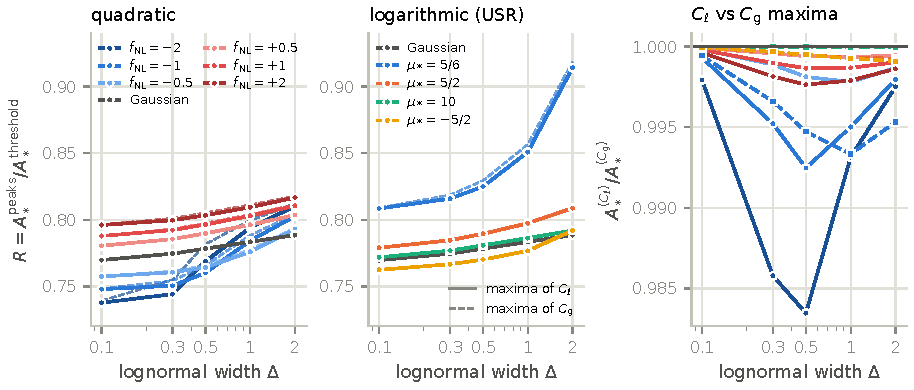
\includegraphics[width=\textwidth]{fig_phase3_ratio}
\caption{The amplitude ratio $R=A_*^{\rm peaks}/A_*^{\rm threshold}$ for $\fpbh=1$ against the
lognormal width $\Delta$, for the quadratic (left) and logarithmic (middle) templates. Solid lines
count maxima of the non-Gaussian compaction $\Cl$, eq.~\eqref{eq:3b}; dashed lines count maxima of
its Gaussian component $\Cg$, eq.~\eqref{eq:3a}. Right: the ratio $A_*^{(\Cl)}/A_*^{(\Cg)}$ of the
amplitudes from the two kinds of maxima, with the colours of the left panels; the logarithmic
family is dashed with square markers. Conventions of table~\ref{tab:conv}, $k_*=10^7\,{\rm Mpc}^{-1}$.}
\label{fig:R}
\end{figure}

\section{Consequences for the PTA tension}\label{sec:pta}

\subsection{Gravitational waves and the NANOGrav 15 likelihood}

For Gaussian $\zeta$ in radiation domination the induced GWs are \cite{Kohri,Espinosa,FIVT23}
\begin{equation}
\Omega_{\rm GW,RD}(k)=\frac16\int_1^\infty\!\dd t\int_0^1\!\dd s\left[\frac{(t^2-1)(1-s^2)}{t^2-s^2}\right]^2
I^2_{t,s}\;\Pz\!\Big(k\frac{t+s}{2}\Big)\Pz\!\Big(k\frac{t-s}{2}\Big),
\label{eq:omegard}
\end{equation}
\begin{equation}
h^2\Omega_{\rm GW}(f)=h^2\Omega_r\,\frac{g_*}{g_*^0}\Big(\frac{g_{*s}}{g_{*s}^0}\Big)^{-4/3}\Omega_{\rm GW,RD}(k),
\end{equation}
with $f=k/2\pi$, $h^2\Omega_r=4.2\times10^{-5}$ and the Standard-Model $g_*(T)$ of
ref.~\cite{Saikawa}. The kernel is \cite{Kohri,FIVT23}
\begin{equation}
\begin{split}
I^2_{t,s}=\frac{288(s^2+t^2-6)^2}{(t^2-s^2)^6}\bigg[&\frac{\pi^2}{4}(s^2+t^2-6)^2\Theta(t-\sqrt3)\\
&+\Big(t^2-s^2-\tfrac12(s^2+t^2-6)\ln\Big|\frac{t^2-3}{3-s^2}\Big|\Big)^2\bigg].
\end{split}
\end{equation}
We rewrite the logarithmic bracket as $(3-s^2)\,g(e)$ with $e=(t^2-s^2)/(3-s^2)$ and
$g=-e^3/12-e^4/12-\dots$, so that the cancellation at $t,s\to1$ is done analytically, and we split
$t$ at the resonance $t=\sqrt3$. A flat spectrum gives $0.8222436\,A^2$ \cite{Kohri}, the Dirac
closed form is recovered, direct two-dimensional integration agrees to $10^{-8}$--$10^{-12}$, and
the infrared $k^3$ tail matches its asymptotic form. This is the spectrum for Gaussian $\zeta$, as
in ref.~\cite{FIVT23}; section~\ref{sec:ngsigw} adds the primordial-NG corrections.

We use the NANOGrav 15-year free spectrum with Hellings--Downs correlations (the lowest 14 bins),
represented by kernel density estimates (KDEs) of the per-bin posteriors in $\log_{10}\rho$
\cite{Lamb,PTArcade}:
\begin{equation}
\ln L=\sum_j\ln p_j(\log_{10}\rho_j),\qquad
\rho_j^2=\frac{H_{100}^2\,h^2\Omega_{\rm GW}(f_j)}{8\pi^4f_j^5T},\qquad T=16.03\,{\rm yr}.
\label{eq:like}
\end{equation}
The KDEs use a compact kernel with bandwidths down to 0.004 dex. Outside the sampled range their
density is floored, and their sparse tails are combs of single-sample spikes. We therefore
regularise them by taking the maximum of each density and its 0.05-dex Gaussian blur
(appendix~\ref{app:kde}). This leaves the bulk unchanged and moves every significance below by
$\le0.14\sigma$. The likelihood reproduces published fits. For $h_c\propto f^{-2/3}$ it gives
$A=2.52^{+0.59}_{-0.61}\times10^{-15}$ (90\%), against $2.4^{+0.7}_{-0.6}\times10^{-15}$ from
NANOGrav \cite{NG15gwb}, and with a free slope $\gamma=3.07^{+0.63}_{-0.56}$, against
$3.2\pm0.6$. For the lognormal SIGW fit with $\Delta$ marginalised it gives
$\log_{10}A=-0.57^{+0.54}_{-0.84}$, against $-0.56^{+0.53}_{-0.74}$ in ref.~\cite{FIVT23}, and for
the broken power law with the shape marginalised $\log_{10}A=-0.84^{+0.79}_{-0.74}$, against
$-0.86^{+0.79}_{-0.65}$, and $\log_{10}k_*=7.95$, against 7.92.

The posterior is taken in $(\log_{10}k_*,\log_{10}A)$, uniform on $[5,10]\times[-3,0]$, for the
same spectral shape as the PBH line. The ``allowed region'' is $A<A_*(k_*)$, where
$\fpbh(A_*)=1$. We quote two measures of its exclusion. The first, $\sigma_P$, is the one-sided
Gaussian equivalent of the posterior mass in the allowed region. The second, $\sigma_{\rm HPD}$,
is the two-sided equivalent of the highest-posterior-density level at which the region is first
reached; this is the definition of ref.~\cite{FIVT23}, whose $1\sigma/2\sigma/3\sigma$ contours
lie at our 69/94/99\% levels. Since $\sigma_{\rm HPD}$ saturates on local features of a lumpy
posterior ridge, we lead with $\sigma_P$. Values above $4\sigma$ lie where the KDEs carry no
information and are quoted only as ``$>4$''. The lines $A_*(k_*)$ for all $k_*$ come from one set
of $\beta$ grids, because the moments depend on $kr$ only.

\subsection{Reproducing the bands of Franciolini et al.}

Figure~\ref{fig:valid} compares our threshold-statistics bands with figure~3 of
ref.~\cite{FIVT23}, read exactly from the vector paths of the arXiv source. Their bands are
reproduced only with two of their conventions: the superhorizon threshold of Musco et al., which
their figure~S3 confirms (appendix~\ref{app:th}), and their $\fpbh$ normalisation. With both, the
agreement for $k_*\ge10^{7.5}\,{\rm Mpc}^{-1}$ is 1--6\% in $A$ for the Gaussian case
(non-linearities only), within 6\% for $\fnl=-2$, within 2.3\% for USR with $\beta=3$, and
8--11\% for the curvaton with $r_{\rm dec}=0.9$. Their bands dip by up to 0.05 dex near
$k_*\simeq10^{6.5}\,{\rm Mpc}^{-1}$, where they include the QCD softening of the formation
parameters and we do not. Putting their own lines on our posterior changes the significance by
$\le0.07\sigma$, so the QCD omission does not matter, as they state.

\begin{figure}[t]
\centering
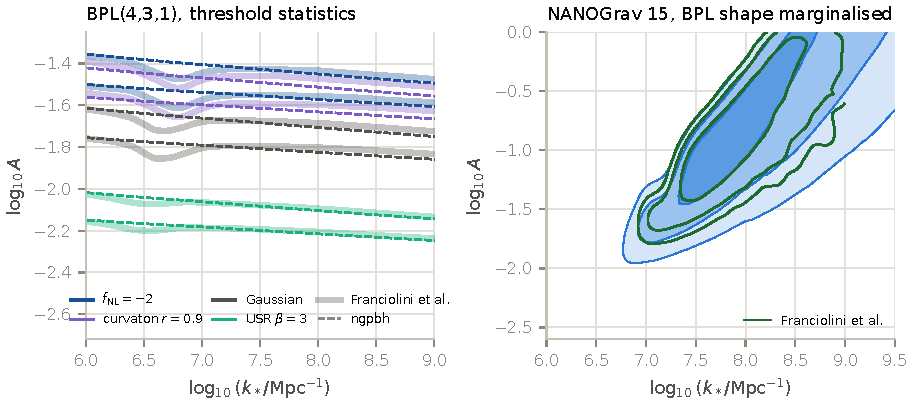
\includegraphics[width=\textwidth]{fig_phase5_validation}
\caption{Comparison with ref.~\cite{FIVT23}. Left: threshold-statistics lines $\fpbh=1$ (upper
of each pair) and $10^{-3}$ (lower) in the plane of the peak scale $k_*$ and amplitude $A$ of
BPL(4,3,1), for four NG templates; wide lines are figure~3 of ref.~\cite{FIVT23} (with QCD
effects), dashed lines are \texttt{ngpbh} (without them), in the conventions of
ref.~\cite{FIVT23}. Right: the NANOGrav 15 posterior with
the BPL shape marginalised (fill: 68.3/95.4/99.7\% highest-posterior-density regions) and the
contours of ref.~\cite{FIVT23}.}
\label{fig:valid}
\end{figure}

\subsection{Exclusion per statistic and NG template}

Table~\ref{tab:pta} gives $\sigma_P$ for threshold statistics and for peaks of the non-Gaussian
compaction in the conventions of ref.~\cite{FIVT23}, and figure~\ref{fig:sigma} shows all
templates. Over the 81 cases with $\sigma_P\le4$, peaks theory adds $\Delta\sigma_P=+0.24$ to
$+0.78$ (median $+0.42$). The amplitude shift itself is nearly uniform, $-0.07$ to $-0.11$ dex
($-0.05$ for the strongest USR tail at $\Delta=2$), and it translates into different $\Delta\sigma$
depending on where the line meets the posterior (figure~\ref{fig:tension}). In the setup of
ref.~\cite{FIVT23}, with the shape-marginalised posterior and the BPL(4,3,1) lines, the Gaussian
case goes from $2.3$ to $2.8\sigma_P$ ($1.4$ to $1.9\sigma_{\rm HPD}$), $\fnl=-2$ from $1.6$ to
$1.9\sigma_P$ and the curvaton from $1.7$ to $2.0\sigma_P$. The USR case with $\beta=3$, which they
place beyond $3\sigma$, gives $3.9\sigma_P$ with threshold statistics and $>4$ with peaks. True NG
peaks and the Gaussian-peak approximation agree to $|\Delta\sigma_P|\le0.04$.

The effect of NG itself is much larger. Relative to the Gaussian case it runs from $-1.2\sigma$
(negative $\fnl$ and the curvaton, for narrow spectra) to well beyond $+2\sigma$ (positive $\fnl$
and USR tails). For $\Delta=2$ the sign of the $\fnl<0$ shift flips, because large negative $\zg$
also produce large compaction.

\begin{table}[t]
\centering\small
\begin{tabular}{lcccc}
\toprule
template & BPL(4,3,1) & LN $\Delta=0.5$ & LN $\Delta=1$ & LN $\Delta=2$\\
\midrule
Gaussian & 2.98\,$\to$\,3.62 & 3.02\,$\to$\,3.52 & 3.54\,$\to$\,$>4$ & 3.84\,$\to$\,$>4$\\
$\fnl=-2$ & 1.87\,$\to$\,2.18 & 1.88\,$\to$\,2.31 & 3.43\,$\to$\,3.84 & $>4$\\
$\fnl=-1$ & 1.98\,$\to$\,2.40 & 1.90\,$\to$\,2.36 & 3.05\,$\to$\,3.46 & 3.89\,$\to$\,$>4$\\
$\fnl=-0.5$ & 2.25\,$\to$\,2.93 & 2.22\,$\to$\,2.89 & 3.09\,$\to$\,3.51 & 3.60\,$\to$\,$>4$\\
$\fnl=+0.5$ & 3.67\,$\to$\,$>4$ & 3.60\,$\to$\,$>4$ & $>4$ & $>4$\\
curvaton $r_{\rm dec}=0.9$ & 2.01\,$\to$\,2.44 & 2.00\,$\to$\,2.43 & 3.09\,$\to$\,3.49 & 3.91\,$\to$\,$>4$\\
USR $\mu_*=5/2$ & 3.53\,$\to$\,$>4$ & 3.49\,$\to$\,3.91 & $>4$ & $>4$\\
$\fnl\ge+1$, USR $\mu_*\le5/6$ & $>4$ & $>4$ & $>4$ & $>4$\\
\bottomrule
\end{tabular}
\caption{Exclusion of the PBH-allowed region by NANOGrav 15: $\sigma_P$, the one-sided Gaussian
equivalent of the posterior mass in the region where $\fpbh<1$, for threshold statistics $\to$
peaks of $\Cl$, eq.~\eqref{eq:3b}. Conventions of ref.~\cite{FIVT23} (threshold without the
transfer function, their $\fpbh$ normalisation), with the same fixed spectral shape in the line
and in the posterior (LN: lognormal).}
\label{tab:pta}
\end{table}

\begin{figure}[t]
\centering
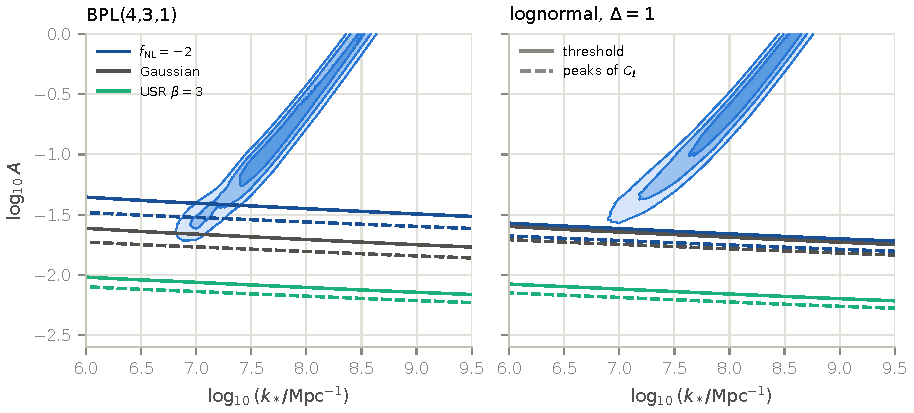
\includegraphics[width=\textwidth]{fig_phase5_tension}
\caption{NANOGrav 15 posteriors in the plane of the peak scale $k_*$ and amplitude $A$
(68.3/95.4/99.7\% highest-posterior-density regions) for BPL(4,3,1) (left) and a lognormal of
width $\Delta=1$ (right), with the $\fpbh=1$ lines from threshold statistics (solid) and peaks of
$\Cl$ (dashed) for $\fnl=-2$, Gaussian $\zeta$ and USR with $\beta=3$, in the conventions of
ref.~\cite{FIVT23}. PBHs are overproduced above each line. Table~\ref{tab:pta} gives the exclusion
$\sigma_P$ of these lines; USR with $\beta=3$ is beyond $4\sigma$ for both statistics.}
\label{fig:tension}
\end{figure}

\begin{figure}[t]
\centering
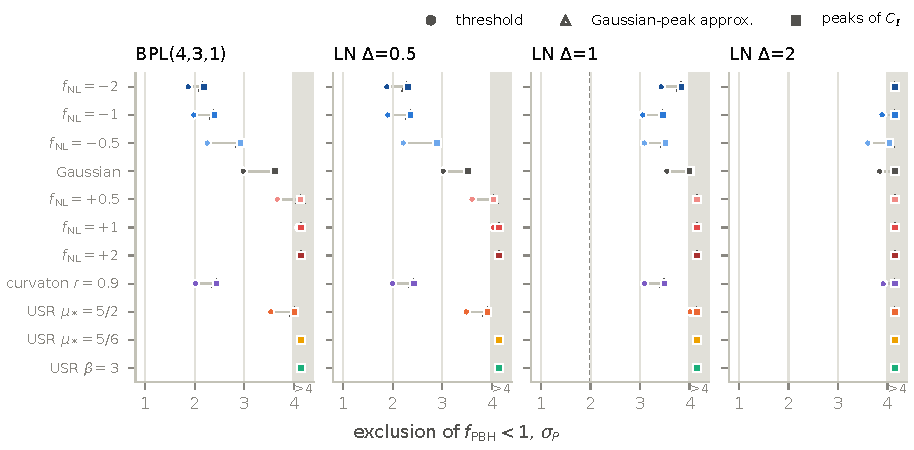
\includegraphics[width=\textwidth]{fig_phase5_sigma}
\caption{Exclusion $\sigma_P$ of the PBH-allowed region by NANOGrav 15 for each NG template and
spectral shape, with threshold statistics (circles), the Gaussian-peak approximation (open
triangles, hidden behind the squares) and peaks of $\Cl$ (squares), in the conventions of
ref.~\cite{FIVT23} (LN: lognormal). Shaded: beyond $4\sigma$, where the KDEs carry no information.}
\label{fig:sigma}
\end{figure}

\subsection{Primordial NG in the induced GWs}\label{sec:ngsigw}

So far the GW spectrum is that of Gaussian $\zeta$, as in ref.~\cite{FIVT23}. For the quadratic
template $\zeta=\zg+F(\zg^2-\langle\zg^2\rangle)$ with $F=3\fnl/5$, the four-point function of
$\zeta$ ends at $F^4$, and the spectrum has seven terms \cite{ALW21} (earlier computations
include refs.~\cite{CPS19,Unal19,AD21}):
\begin{equation}
\Omega_{\rm GW,RD}=A^2T_2+F^2A^3\,(T_{\rm hyb}+T_C+T_Z)+F^4A^4\,(T_{\rm red}+T_{\rm pl}+T_{\rm np}).
\label{eq:ngterms}
\end{equation}
For $\Pz^{\rm g}=A\,s(k/k_*)$ each term depends on $k/k_*$ only, and $A$ is the amplitude of the
Gaussian component, as in the PBH lines. All seven follow from
\begin{equation}
\Omega_X=\frac{k^3c_X}{12\pi^2}\int\prod_{\rm loops}\frac{\dd^3q}{(2\pi)^3}\,
{\rm Re}\big[z_1^2\bar z_2^2\big]\,J_{12}\prod_iP(|\bm m_i|),\qquad
J_{12}=\tfrac12\big(I_{A1}I_{A2}+I_{B1}I_{B2}\big).
\end{equation}
Here $z=(q_x+iq_y)/k$ is the transverse momentum of a GW vertex ($\bm k=k\hat z$). $J_{12}$ is the
oscillation average of the product of the late-time transfer functions
$I=(I_A\sin x+I_B\cos x)/x$ of the two vertices \cite{Kohri}, and $J_{11}$ is the kernel above. The
$\bm m_i$ are the momenta that carry a power spectrum, $P(m)=2\pi^2\Pz^{\rm g}(m)/m^3$, and
$c_X=2$, 8, 16, 16, 8, 32, 16 for the Gaussian, hybrid, C, Z, reducible, planar and nonplanar
terms. These reproduce the prefactors $2^5$, $2^7F^2$, $2^8F^2$, $2^8F^2$, $2^7F^4$, $2^9F^4$,
$2^8F^4$ of ref.~\cite{ALW21}.

The disconnected terms are the Gaussian functional of $P_{\rm g}+P_2$, with the one-loop spectrum
$\Pz^{(2)}=F^2A^2s_2$: we compute $T_{\rm hyb}=2\,\Omega_{\rm bil}[s,s_2]$ and
$T_{\rm red}=\Omega_{\rm G}[s_2]$ with the quadrature above. The connected terms are five- and
eight-dimensional, and we evaluate them with randomised quasi-Monte Carlo over the spectral
momenta. $L$ of the $L+1$ momenta $\bm m_i$ are drawn from the spectrum, and the last follows from
momentum conservation. The choices of which momentum is fixed are combined with the balance
heuristic, so that the weights stay bounded when a momentum becomes soft. For broad spectra, pairs
of nearly independent vertices dominate the variance: ${\rm Re}[z_1^2\bar z_2^2]\propto\cos2\phi$
averages to zero but scatters. We therefore average each sample over rotations about $\bm k$ of
one spectral momentum (for the planar term, of two, independently). The rotations preserve the
measure and every weight, so the estimate stays unbiased, and the oscillation cancels.

The Monte Carlo reproduces the quadrature of the Gaussian, hybrid and reducible terms in 72
comparisons with an rms pull of 0.97. All six NG terms agree with figure~4 of ref.~\cite{ALW21},
read from the vector paths of the arXiv source (figure~\ref{fig:ngvalid}): for lognormal widths
1/5 and 1/10 the agreement is within 3\% of each curve's maximum, including the sign changes of
$T_Z$ and the negative $T_{\rm np}$.

For other templates, $\zeta=\zg+F\zg^2+G\zg^3+\dots$, only $F$ and $G$ enter at $O(A^3)$. $G$
enters through the power renormalisation $P\to(1+6G\sigma^2)P$, i.e.\ $+12G\sigma^2A^2T_2$; the
$g_{\rm NL}$-type trispectrum vanishes under the azimuthal integral \cite{GPRW22,Perna24}.
$O(A^4)$ would need $G^2$, $F^2G$ and $FH$ terms, so we truncate the curvaton ($F=-0.62$,
$G=0.32$ \cite{SVW06}) and the USR maps ($F=1/2\mu_*$, $G=1/3\mu_*^2$) at $A^3$. The quadratic
template is exact at $A^4$.

\begin{figure}[t]
\centering
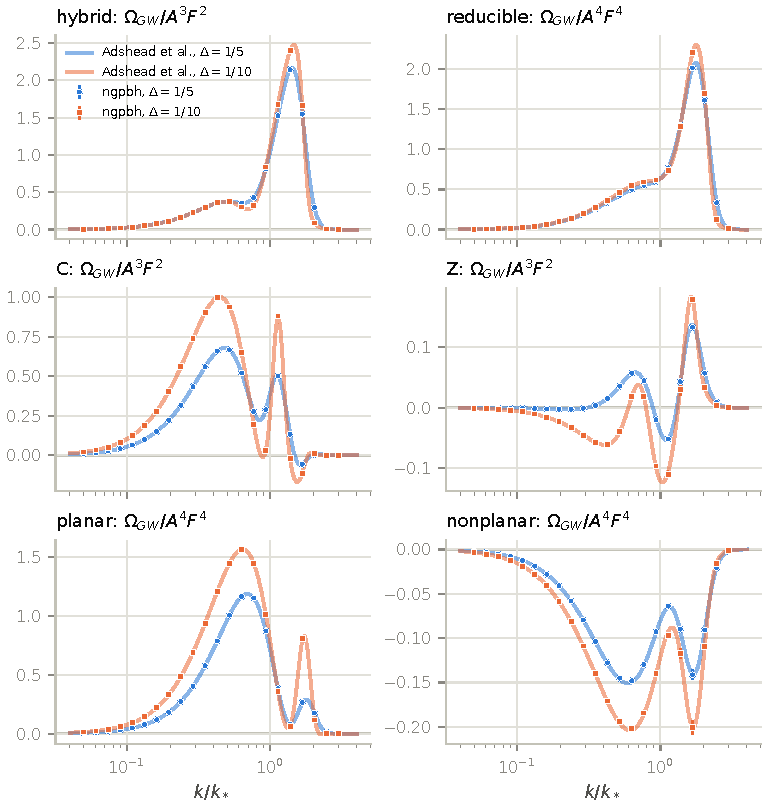
\includegraphics[width=0.84\textwidth]{fig_sigw_ng_validation}
\caption{The six NG terms of the induced GW spectrum, eq.~\eqref{eq:ngterms}, for lognormal peaks
of width $\Delta=1/5$ and $1/10$ with $A=F=1$: \texttt{ngpbh} (markers; the Monte Carlo errors are
smaller than the markers)
against figure~4 of Adshead, Lozanov and Weiner \cite{ALW21} (lines, read from the vector paths
of the arXiv source).}
\label{fig:ngvalid}
\end{figure}

Relative to $T_2$ the corrections are large (figure~\ref{fig:ngterms}). In the NANOGrav band of
the posterior bulk, $k/k_*\simeq0.02$--0.3, the ratio $T_3/T_2$ is 2--6. It grows with the width of
the peak, because the one-loop spectrum collects the whole variance $\sigma^2=A$ while the peak
value of a broad lognormal is low. For $|\fnl|=2$, $\Omega_{\rm GW}$ at fixed $A$ is therefore
10--40\% larger near the PBH lines ($A\simeq0.03$--0.05), and in the posterior bulk it is more than
doubled. The posterior median of $\log_{10}A$ moves down by 0.08--0.18 dex for $|\fnl|=2$, by
0.04--0.11 for the curvaton, and by $\le0.02$ for $|\fnl|=0.5$.

\begin{figure}[t]
\centering
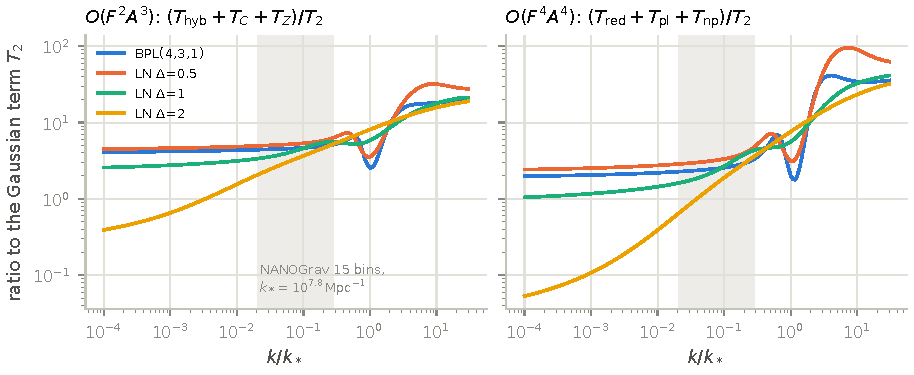
\includegraphics[width=\textwidth]{fig_sigw_ng_terms}
\caption{The NG corrections to the induced GW spectrum relative to the Gaussian term $T_2$, for
each spectral shape: the $O(F^2A^3)$ terms (left) and the $O(F^4A^4)$ terms (right) of
eq.~\eqref{eq:ngterms}, for the quadratic template with $F=3\fnl/5$. Shaded: the 14 NANOGrav bins
for $k_*=10^{7.8}\,{\rm Mpc}^{-1}$, near the posterior median.}
\label{fig:ngterms}
\end{figure}

The PBH-allowed region lies at small $A$, so the exclusion weakens (table~\ref{tab:ngsigw},
figure~\ref{fig:ngsigw}). Over the cases with $\sigma_P\le4$, $\sigma_P$ drops by 0.10--0.26 for
$\fnl=\pm2$, by 0.03--0.20 for the curvaton, by $\le0.09$ for $|\fnl|=1$, and by $\le0.03$ for
$|\fnl|=0.5$ and USR $\mu_*=5/2$. The statistics shift is unchanged: threshold $\to$ peaks adds
$+0.23$ to $+0.67$ (median $+0.39$), against $+0.24$ to $+0.68$ (median $+0.42$) with the Gaussian
spectrum, and none of the 66 pairs changes by more than $\pm0.10$. The truncation matters little:
dropping the $A^4$ terms of the quadratic template, or adding the $F^4A^4$ terms to the others,
moves $\sigma_P$ by $\le0.02$. The GW part of the NG effect thus relieves the tension for either
sign of $\fnl$, by at most $0.26\sigma$, while the PBH part shifts $\sigma_P$ by $-1.2$ to beyond
$+2\sigma$.

\begin{table}[t]
\centering\small
\begin{tabular}{llccc}
\toprule
template & GW spectrum & BPL(4,3,1) & LN $\Delta=0.5$ & LN $\Delta=1$\\
\midrule
$\fnl=-2$ & Gaussian & 1.87\,$\to$\,2.18 & 1.88\,$\to$\,2.31 & 3.43\,$\to$\,3.84\\
 & with NG & 1.73\,$\to$\,2.05 & 1.73\,$\to$\,2.11 & 3.25\,$\to$\,3.67\\
$\fnl=-1$ & Gaussian & 1.98\,$\to$\,2.40 & 1.90\,$\to$\,2.36 & 3.05\,$\to$\,3.46\\
 & with NG & 1.94\,$\to$\,2.34 & 1.85\,$\to$\,2.30 & 2.99\,$\to$\,3.42\\
$\fnl=-0.5$ & Gaussian & 2.25\,$\to$\,2.93 & 2.22\,$\to$\,2.89 & 3.09\,$\to$\,3.51\\
 & with NG & 2.24\,$\to$\,2.91 & 2.20\,$\to$\,2.87 & 3.07\,$\to$\,3.50\\
curvaton $r_{\rm dec}=0.9$ & Gaussian & 2.01\,$\to$\,2.44 & 2.00\,$\to$\,2.43 & 3.09\,$\to$\,3.49\\
 & with NG & 1.92\,$\to$\,2.30 & 1.88\,$\to$\,2.26 & 2.95\,$\to$\,3.38\\
USR $\mu_*=5/2$ & Gaussian & 3.53\,$\to$\,$>4$ & 3.49\,$\to$\,3.91 & $>4$\\
 & with NG & 3.51\,$\to$\,4.00 & 3.47\,$\to$\,3.90 & 3.99\,$\to$\,$>4$\\
\bottomrule
\end{tabular}
\caption{Effect of primordial NG in the induced GWs on the exclusion: $\sigma_P$, the one-sided
Gaussian equivalent of the posterior mass in the PBH-allowed region, for threshold statistics
$\to$ peaks of $\Cl$, with the Gaussian induced GW spectrum (as in table~\ref{tab:pta}) and with
its primordial-NG corrections (each template with its own posterior). $\fpbh=1$, conventions of
ref.~\cite{FIVT23}. The other templates are beyond $4\sigma$ with either spectrum.}
\label{tab:ngsigw}
\end{table}

\begin{figure}[t]
\centering
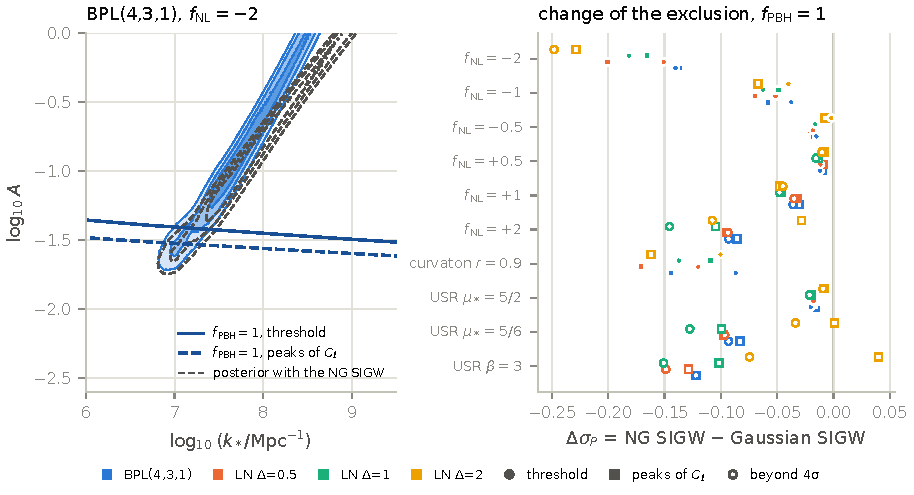
\includegraphics[width=\textwidth]{fig_phase5_ngsigw}
\caption{Effect of primordial NG in the induced GWs. Left: the NANOGrav 15 posterior for
BPL(4,3,1) with the Gaussian induced GW spectrum (fill) and with its NG corrections for
$\fnl=-2$ (dashed; 68.3/95.4/99.7\% highest-posterior-density regions), with the $\fpbh=1$ lines.
Right: the change of $\sigma_P$ from the NG corrections for every template (rows), spectral shape
(colours) and statistic (circles: threshold statistics, squares: peaks of $\Cl$); open symbols lie
beyond $4\sigma$. Conventions of ref.~\cite{FIVT23}, $\fpbh=1$.}
\label{fig:ngsigw}
\end{figure}

\subsection{Robustness}\label{sec:robust}

Table~\ref{tab:robust} varies one analysis choice at a time. The statistics shift survives every
change: it is $+0.2$ to $+0.8\sigma$ across the peak-normalisation conventions in use, and $+0.8$
to $+1.3\sigma$ with the high-peak formula. The absolute significance depends mainly on the
frequency range, as 5, 14 or 30 bins move it by $-1.5$ to $+1\sigma$: the part of the posterior
nearest the allowed region, $k_*\simeq10^7\,{\rm Mpc}^{-1}$, places the GW peak at 10--20 nHz, and
the bins above it bound it. Among the other conventions, the horizon-crossing transfer function in
the threshold moves the significance by $-0.2$ to $-1.0\sigma$, the entropy-conserving $\fpbh$
normalisation by $-0.15$ to $-0.4\sigma$, $\fpbh=10^{-3}$ instead of 1 by $+0.4$ to $+0.8\sigma$,
and a $\pm5\%$ change of $C_{\rm th}$ in both statistics by up to $\pm0.54\sigma$ for the Gaussian,
$\fnl<0$ and curvaton templates. Fixing the spectral shape raises the significance relative to
marginalising over it (Gaussian BPL: $3.0$ against $2.3\sigma_P$), because the fixed BPL(4,3,1)
has a steep causality tail that disfavours the low-$k_*$ corner closest to the allowed region.

\begin{table}[t]
\centering\small
\begin{tabular}{lcc}
\toprule
change from the reference & $\Delta\sigma_P$, threshold $\to$ peaks & max.\ change of $\sigma_P$\\
\midrule
none (14 bins, KDE blur 0.05 dex) & $+0.31$ to $+0.68$ & ---\\
prior $\log_{10}k_*\in[6,9]$, or $\log_{10}A\ge-4$ & unchanged & 0.00\\
posterior grid twice as fine & unchanged & 0.00\\
KDE blur 0, 0.03 or 0.10 dex & $+0.30$ to $+0.72$ & 0.14\\
5 frequency bins (2--10 nHz) & $+0.27$ to $+0.72$ & 1.45\\
30 frequency bins (2--59 nHz) & $+0.23$ to $+0.55$ & 1.06\\
peak volume $(2\pi)^{3/2}r^3$ & $+0.40$ to $+0.81$ & 0.14\\
Press--Schechter factor 2 & $+0.27$ to $+0.59$ & 0.09\\
\texttt{pbhstat} v0.0.6 normalisation & $+0.16$ to $+0.39$ & 0.33\\
high-peak formula \cite{Iovino24} (indicative) & $+0.82$ to $+1.29$ & 0.65\\
$C_{\rm th}\times0.95$ (five templates) & $+0.42$ to $+0.75$ & 0.54\\
$C_{\rm th}\times1.05$ (five templates) & $+0.23$ to $+0.72$ & 0.54\\
\bottomrule
\end{tabular}
\caption{Robustness of the PTA significances to one analysis choice at a time, for BPL(4,3,1)
and lognormals with $\Delta=0.5$ and 1, over seven NG templates (cases with $\sigma_P\le4$); the
$C_{\rm th}$ rows cover the Gaussian, $\fnl=-2,-1,-0.5$ and curvaton templates. Reference: the
conventions of ref.~\cite{FIVT23} and the uniform prior $\log_{10}k_*\in[5,10]$,
$\log_{10}A\in[-3,0]$.}
\label{tab:robust}
\end{table}

\subsection{An astrophysical background}\label{sec:smbhb}

So far the SIGW is the whole signal. We now add a power law from supermassive black hole binaries
(SMBHBs), whose timing residuals add to those of the SIGW,
$\rho_j^2\to\rho_j^2+A_B^2(f_j/f_{\rm yr})^{3-\gamma_B}/(12\pi^2f_j^3T)$, with NANOGrav's
astrophysical prior on $(\log_{10}A_B,\gamma_B)$, a two-dimensional Gaussian with mean
$(-15.6,4.7)$ \cite{NG15np}, and marginalise over it. SIGW plus SMBHB is preferred over the SMBHB
alone by Bayes factors of 94--105 for BPL(4,3,1) and the lognormals with $\Delta\le1$, and 38 for
$\Delta=2$, of the same order as NANOGrav's 23--59 for their SIGW templates \cite{NG15np}.

The PBH-allowed region now contains the solutions in which the SMBHB alone explains the signal.
As a result $\sigma_P$ is capped at 2.3--2.8$\sigma$ for every template, or 2.0--2.5$\sigma$ if
the prior on $\log_{10}A$ extends to $-4$, and the templates that relieve the tension stay at
1.8--2.6$\sigma$. The statistics shift drops to $+0.04$ to $+0.39\sigma$ (median $+0.26$, against
$+0.43$ without the SMBHB on the same grid). The profile $\Delta\chi^2$, which does not depend on
the prior range, keeps the shift where the PBH line cuts the SIGW posterior (7.7 to 12.5 for the
Gaussian BPL) and saturates at $\simeq18$, the cost of explaining the signal with the SMBHB alone.

\section{Discussion}\label{sec:disc}

The question we set out to answer is whether the gap between threshold statistics and peaks
theory, once local NG is included for broad spectra, changes how strongly PBH overproduction
disfavours a scalar-induced explanation of the PTA signal. It does, modestly and uniformly. Peaks
theory lowers the overproduction line by about 0.1 dex for every NG template, which strengthens
the exclusion by $\simeq0.4\sigma$, or 0.2--0.8$\sigma$ depending on the peak normalisation. In the
framing of ref.~\cite{Iovino24} the same effect relaxes the PTA bound on $\fpbh$: at fixed $A$
peaks theory predicts more PBHs, so the PTA bound on $A$ allows a larger $\fpbh$, while the line
$\fpbh=1$ moves down into the PTA posterior. Their high-peak normalisation ($R\approx0.6$--0.67)
enlarges both effects.

The NG dependence of the gap cancels almost completely, the double ratio being 1 to about 4\%, so
NG and the choice of statistics add rather than interact. Negative $\fnl$ and the curvaton remain
the ways to relieve the tension, but peaks theory takes back 0.3--0.5$\sigma$ of the relief. NG in
the induced GWs adds power at fixed $A$; it relieves the tension by up to $0.26\sigma$ for
$|\fnl|\le2$ and does not change the gap between the statistics. None of the conclusions of
ref.~\cite{FIVT23} changes qualitatively: their remark on peaks theory is correct, and now
quantified.

For an absolute statement about the PTA tension, the larger uncertainties lie elsewhere. The
largest is an astrophysical SMBHB background: with NANOGrav's prior it caps every exclusion at
2.3--2.8$\sigma$ and reduces the statistics shift to 0.04--0.39$\sigma$. Among the analysis
choices, the frequency range of the fit, the treatment of the collapse threshold and the $\fpbh$
normalisation each move the significance by about as much as the choice of statistics, or more.
All three are rarely stated, and we recommend quoting them with any PBH bound on the PTA signal,
together with the peak normalisation when peaks theory is used. On the theory side, the
Gaussian-peak approximation is adequate for the PTA question (to $0.04\sigma$), although it
miscounts peaks by up to 18\%.

Our results rest on several simplifications. We assume spherical symmetry for the compaction of a
peak \cite{Young22} and use the mean profile, as the literature we compare with does; profile
dispersion can matter for negative NG \cite{Escriva26}. The collapse threshold follows from the
power spectrum and is the same for every NG template, although NG also deforms the typical profile
and hence the threshold \cite{KMR19,ETYY22}; a $\pm5\%$ change moves $\sigma_P$ by up to
$0.54\sigma$ and $R$ by $\le0.3\%$ ($\le6\%$ for the curvaton, section~\ref{sec:R}). Each scale is
counted separately, without a cloud-in-cloud correction. We neglect QCD effects on the formation
parameters \cite{MJY23,FMPU22} and on the GW spectrum \cite{ATU21,BDF23}, truncate the NG series of
the GW spectrum at $A^3$ for the curvaton and USR maps, and use the free-spectrum refit rather
than the full PTA likelihood; the SMBHB background is a power law with NANOGrav's prior. These
choices are common to both statistics, so the comparison between them is like-for-like, while the
absolute numbers carry the systematics of table~\ref{tab:robust}. Finally, $R$ refers to BBKS
maxima of the compaction at fixed scale, the prescription that differs from threshold statistics
only by the peak condition. Peaks of $\zeta$ with typical profiles \cite{Yoo18,Yoo20,Kitajima}
and the non-linear statistics of ref.~\cite{GS20} define the abundance differently; we have not
computed $R$ for them in our conventions, but section~\ref{sec:R} quotes what the literature
finds for Gaussian $\zeta$.

\section{Conclusions}\label{sec:concl}

We have constructed peaks theory with local NG for broad spectra on the compaction function, as
the exact counterpart of threshold statistics. Maxima of the non-Gaussian compaction are maxima of
a shifted Gaussian field, corrected by a rank-one term, eq.~\eqref{eq:3b}, and Monte Carlo and
lattice counts confirm this. Peaks require 18--26\% smaller amplitudes than threshold statistics,
and this ratio is almost independent of NG for $|\fnl|\le2$: a threshold-statistics amplitude
converts to peaks theory as $A_*^{\rm peaks}\simeq R_{\rm Gauss}A_*^{\rm threshold}$, with
$R_{\rm Gauss}=0.783+0.0066\ln\Delta$ for the lognormal and 0.775--0.778 for the BPL, to about 4\%.

For NANOGrav 15 this strengthens the exclusion of a scalar-induced explanation by
0.2--0.8$\sigma$ for every NG template, or by 0.04--0.39$\sigma$ with an SMBHB background, which
caps the exclusion at 2.8$\sigma$. The effect is smaller than that of NG itself for
$|\fnl|\gtrsim1$, and comparable to three analysis conventions, which we have quantified. The
primordial-NG corrections to the induced GW spectrum, with all seven terms, relieve the tension by
up to $0.26\sigma$ for $|\fnl|\le2$ and leave the gap between the statistics unchanged. The code
\texttt{ngpbh} implements every piece and reproduces published results: \texttt{pbhstat}, Ferrante
et al., Franciolini et al.\ and Adshead et al.

\appendix

\section{Peaks of the non-Gaussian compaction: the rank-one factor}\label{app:3b}

At a stationary point of $\Cl$, write $H_\lambda=\nabla\nabla Y_\lambda$ and $\bm g=\nabla\zr$,
with $\bm g\sim\mathcal N(0,v\mathbb I)$ independent of $H_\lambda$. The exact density is
\begin{equation}
n(c,z)=P_{\rm G}(c,z)\Big(\frac{3}{2\pi\sigma^2_{1,\lambda}}\Big)^{3/2}
\E\big[|\det(H_\lambda+\kappa\bm g\bm g^T)|\,\Theta_s\big],
\end{equation}
where $\Theta_s$ requires negative (positive) definiteness for $s=+1$ ($-1$). For $H\prec0$ the
matrix determinant lemma gives
$\det(-H-\kappa\bm g\bm g^T)=\det(-H)\,[1-\kappa\,\bm g^T(-H)^{-1}\bm g]$, which is linear in
$\kappa|\bm g|^2$. Averaging over the direction and length of $\bm g$ gives
$v\,\det(-H){\rm tr}(-H)^{-1}=v\,e_2(-H)$. In the BBKS shape variables $e_2=x^2/3-(3y^2+z^2)/3$,
so $f_2(x)=\E[e_2\Theta|x]$ follows from the same two-dimensional integral as $f$; that integral
reproduces the BBKS function $f$ to $10^{-10}$. The interior part of the first-order factor is
then exactly $1-\tau R_2$. For $\tau>0$ maxima can only be lost, so $1-\tau R_2$ is a lower bound;
for $\tau<0$, configurations that become maxima add a positive $\mathcal O(\tau^2)$ term. The
Monte Carlo bounds the remainder at 0.85\% at the most extreme node tested, a shift of 0.02\% in
$A_*$.

\section{The PBH abundance from entropy conservation}\label{app:fpbh}

After formation at temperature $T$, the PBH number per entropy is conserved, so
$\rho_{\rm PBH,0}=\frac34\beta\,(g_*/g_{*s})\,T\,s_0$, with $s_0=\frac{2\pi^2}{45}g_{*s}^0T_0^3$.
Here $\beta(M_H)$ is the fraction of the energy density at formation that collapses into PBHs,
weighted by $M/M_H=\mathcal K(C-C_{\rm th})^\gamma$ as in eq.~\eqref{eq:betath}. With
$M_H=4\pi M_P^2/H$ and $H=\pi(g_*/90)^{1/2}T^2/M_P$ this gives
\begin{equation}
\fpbh=\frac{1}{\Omega_{\rm DM}}\int\dd\ln M_H\Big(\frac{M_H}{\Mo}\Big)^{-1/2}
\Big(\frac{g_*}{106.75}\Big)^{3/4}\Big(\frac{g_{*s}}{106.75}\Big)^{-1}\frac{\beta(M_H)}{1.0\times10^{-8}},
\end{equation}
for $h=0.674$ and $\Omega_{\rm DM}h^2=0.12$. It agrees with Carr et al.~\cite{Carr10} to 2\%, and
with the exact expression of ref.~\cite{CK20} (their eq.~II.3, written in terms of $M_H$) to
1.5\%.

The constant $7.9\times10^{-10}$ in eq.~(14) of ref.~\cite{FIVT23} makes $\fpbh$ 12.7 times
larger. It equals $[2.4\,(M_{\rm eq}/\Mo)^{1/2}]^{-1}$ with $M_{\rm eq}=2.8\times10^{17}\,\Mo$, the
normalisation of the approximation $\fpbh\simeq2.4\,\beta\,(M_{\rm eq}/M)^{1/2}$ of
ref.~\cite{CK20}, which is already a fraction of the dark matter. Dividing it by $\Omega_{\rm DM}$
once more gives a factor 3.8, and the approximation itself exceeds the entropy-conserving result by
3.4 when $M$ is identified with $M_H$. The form $(M_{\rm eq}/M_H)^{1/2}\beta/\Omega_{\rm DM}$ drops
the factor $\Omega_m$ and the heating of the radiation by the changes of $g_{*s}$ after formation,
and is 3--5 times larger. Both lower the amplitude for $\fpbh=1$ by $\ln(\text{factor})/|\ln\beta|$,
i.e.\ 8--12\% at $|\ln\beta|\simeq21$.

\section{The collapse threshold of Franciolini et al.}\label{app:th}

Figure~S3 of ref.~\cite{FIVT23} plots $\delta_{\rm th}$ from the Musco et al.\ prescription
against the lognormal width and against the UV slope $\beta$ of BPL(4,$\beta$,1). The figure is
vector graphics in the arXiv source, so we read the curves exactly and compare them with three
readings of the prescription (figure~\ref{fig:th}). Without a transfer function we reproduce their
curves to $\le0.0002$ for $0.1\le\Delta\le1$ and to $\le0.0016$ for $1.9\le\beta\le3$. With $T$
at $\eta=\hat r_m/10$, the superhorizon smoothing of Musco et al., the agreement is $\le0.0005$
and $\le0.0012$. With $T$ at horizon crossing, which is what the notation $T(k,r_m)$ of their
eqs.~(S4)--(S5) suggests, the curves are off by up to 0.08. For $\beta<2$ the integrals without
$T$ converge only conditionally, because the UV tail falls like $k^{-\beta}$; their curve has a
kink at $\beta\simeq1.8$ and lies up to 0.007 below ours there. Their plotted $\alpha_s$ for the
BPL is not the one behind their plotted $\delta_{\rm th}$ through their eq.~(S6), while for the
lognormal both curves agree with ours. Their thresholds are therefore those of Musco et al., and
the conclusions of ref.~\cite{FIVT23} do not depend on the notation.

\begin{figure}[t]
\centering
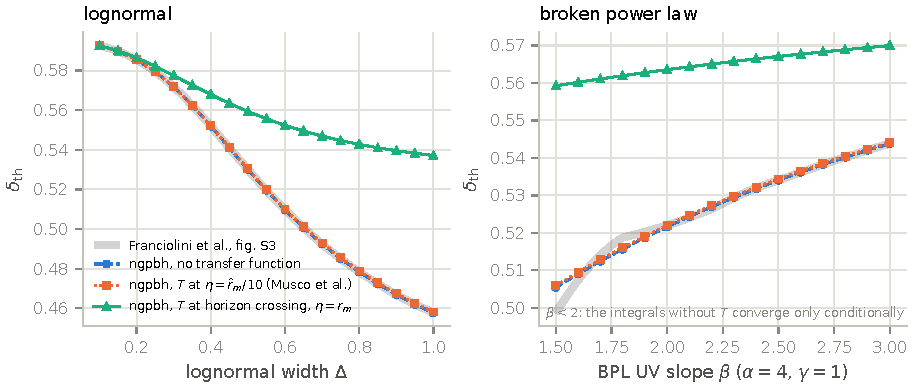
\includegraphics[width=\textwidth]{fig_threshold_check}
\caption{The collapse threshold $\delta_{\rm th}$ of figure~S3 of ref.~\cite{FIVT23} (wide gray),
read from its vector paths, against the lognormal width $\Delta$ (left) and the UV slope $\beta$
of BPL(4,$\beta$,1) (right), compared with \texttt{ngpbh} for three readings of the Musco et al.\
prescription: without the transfer function, with Musco et al.'s superhorizon smoothing
($\eta=\hat r_m/10$) and with the horizon-crossing transfer function.}
\label{fig:th}
\end{figure}

\section{Free-spectrum density estimates}\label{app:kde}

The per-bin densities distributed with PTArcade \cite{PTArcade,Lamb} are Epanechnikov KDEs on a
grid of $10^4$ points in $\log_{10}\rho$. The kernel has compact support, so the density is
exactly zero (stored as $\ln p=-36$) outside the range of the samples, and within the sparse tails
it alternates between single-sample spikes and zero. The two most constraining bins (3.9 and
5.9 nHz) have almost no low-$\rho$ tail. Tail probabilities beyond $\sim2.5\sigma$ are therefore
lumpy and cliff-like. We replace each density by the maximum of itself and its convolution with a
0.05-dex Gaussian, which leaves the bulk unchanged and fills the holes. Table~\ref{tab:robust}
shows that the result changes by at most $0.14\sigma$ between no blur and 0.10 dex.

\acknowledgments

This work made extensive use of the AI assistant Claude (Anthropic), through Claude Code, to write
and test the code \texttt{ngpbh}, run the numerical checks and draft the text. The author is
responsible for the content of this paper.

\section*{Code and data availability}

The code \texttt{ngpbh} (MIT licence) and the source of this paper are archived at Zenodo, version
0.7.1, \href{https://doi.org/10.5281/zenodo.23661308}{doi:10.5281/zenodo.23661308};
\href{https://doi.org/10.5281/zenodo.23624506}{doi:10.5281/zenodo.23624506} resolves to the latest
version. The archive contains the scripts that produce every table and figure
(\texttt{README.md}), 96 unit tests, the digitised figures~3 and S3 of ref.~\cite{FIVT23} and
figure~4 of ref.~\cite{ALW21}, and the tables of the NG terms of the induced GW spectrum per
spectral shape. The NANOGrav 15 free-spectrum densities are those of PTArcade (Zenodo record
10495907) and are downloaded with an MD5 check.

\bibliographystyle{JHEP}
\bibliography{refs}

\end{document}
